\documentclass[10pt,twocolumn,letterpaper]{article}

\usepackage{cvpr}
\usepackage{times}
\usepackage{epsfig}
\usepackage{graphicx}
\usepackage{amsmath}
\usepackage{amssymb}

% Include other packages here, before hyperref.

% If you comment hyperref and then uncomment it, you should delete
% egpaper.aux before re-running latex.  (Or just hit 'q' on the first latex
% run, let it finish, and you should be clear).
\usepackage[breaklinks=true,bookmarks=false]{hyperref}

\cvprfinalcopy % *** Uncomment this line for the final submission

\def\cvprPaperID{****} % *** Enter the CVPR Paper ID here
\def\httilde{\mbox{\tt\raisebox{-.5ex}{\symbol{126}}}}

% Pages are numbered in submission mode, and unnumbered in camera-ready
%\ifcvprfinal\pagestyle{empty}\fi
\setcounter{page}{4321}
\begin{document}

%%%%%%%%% TITLE
\title{Machines are Among Us}

\author{Zach Minot\\
Georgia Institute of Technology\\
2nd Year Undergraduate, CS\\
{\tt\small zjminot@gatech.edu}
% For a paper whose authors are all at the same institution,
% omit the following lines up until the closing ``}''.
% Additional authors and addresses can be added with ``\and'',
% just like the second author.
% To save space, use either the email address or home page, not both
\and
Charles Gunn\\
Georgia Institute of Technology\\
2nd Year Undergraduate, CS \& Math\\
{\tt\small cgunn30@gatech.edu}
}

\maketitle
%\thispagestyle{empty}

%%%%%%%%% ABSTRACTcommunicate
\begin{abstract}
   The ABSTRACT is to be in fully-justified italicized text, at the top
   of the left-hand column, below the author and affiliation
   information. Use the word ``Abstract'' as the title, in 12-point
   Times, boldface type, centered relative to the column, initially
   capitalized. The abstract is to be in 10-point, single-spaced type.
   Leave two blank lines after the Abstract, then begin the main text.
   Look at previous CVPR abstracts to get a feel for style and length.
\end{abstract}

%%%%%%%%% BODY TEXT
\section{Introduction}
To what extent can neural network models communicate with each other and discover
each other's identity? How would they use this information in a competitive setting?
For example, in a social deduction game, players attempt to uncover each other's
hidden allegiance---typically with one "good" team and one "bad" team.
Players must utilize deductive reasoning to find the truth or instead
lie to keep their role hidden. In this paper, we explore 
if neural networks can be successfully trained to
compete in a scenario such as this, and how would the opposing parties interact
during the period of debate.
\subsection{Among Us}
Among Us is a currently popular social deduction game,
where the "imposters" attempt to sabotage and kill all of the "crewmates". Crewmmates have
to complete tasks and figure out who the imposters are and eliminate them before the imposters
win.
At certain points in the game, after periods of no direct communication, players 
debate the roles of each individual based on information previously acquired through
their personal experience. At the end of this discussion, every player votes on a single
player to be eliminated. The player with the most votes is eliminated, and if there
is a tie, no one is voted out. We chose to emulate this game based on
the overall simplicity of the two roles and the requirement of communication
for either party to succeed. If the crew do not exchange information 
and all vote the same person, 
the vote could result in a tie or a crew being eliminated.
If the imposters do not bluff, the crew can easily spot the liars among the group. 
This provides ample room to explore and experiment with the communication between
the two opposing parties.
\subsection{Adverserial Networks}
Within this design space, there are adversarial parties working against each other.
In the deep learning realm, adversarial situations appear in adversarial examples~\cite{AdverserialEx} and within GANs (generative adversarial networks)
~\cite{NIPS2014_5ca3e9b1}
In particular, the latter often designs a contest between two neural networks, in the form
of a zero-sum game.
We build upon these concepts and foundations in our work.
\subsection{Multi-agent Communication}
Inherently, a social deduction game requires multiple agents to be trained and contested.
This has been explored within the deep learning problem space with multi-agent subproblems.
Both cooperative~\cite{DBLP:journals/corr/FoersterAFW16}~\cite{DBLP:journals/corr/FoersterAFW16a} 
and adversarial ~\cite{DBLP:journals/corr/AbadiA16} communication has been experimented with,
showing that models can effective share and also selectively protect information.
We reference these approaches we generate active adversarial communication between 
neural network models.
\section{Approach}
We deconstructed a standard voting round of Among Us into three stages: 
communicationless information gain,
argument and debate, and the final vote. Building off of this, we decided 
to break our standard player model into a perception stage, 
communication stage, and voting stage. Each satge feeds into the next until the final
vote occurs to eliminate one of the models within the communicating group.
\subsection{Deductive Situation}
During the period of communication in Among Us, the crew must do tasks
and gain information while the imposters must sabotage and kill the crew. We decided
to simplify the game by both removing the tasks and killing and making the entire
perception of each player predetermined.
\subsection{Modeling Interpretation and Communication}
\begin{figure*}
   \begin{center}
      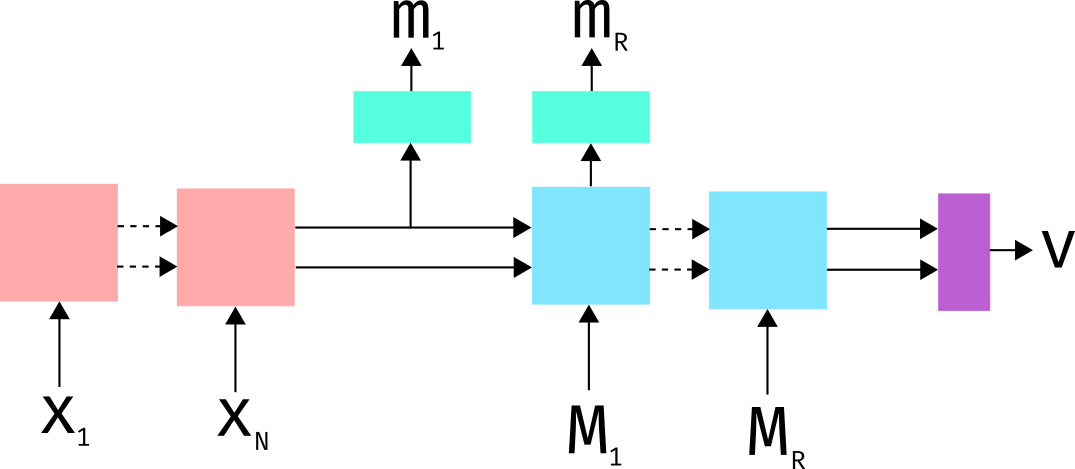
\includegraphics[width=0.8 \textwidth]{img/model.png}
   \end{center}
      \caption{Diagram of the Agent model. The red section is the perception LSTM,
      which takes in a sequence of events. The blue section is the communication
      LSTM, which recieves messages, and generates messages using the green MLP.
      Finally, the purple section is the voting MLP, which produces the agent's
      vote vector.}
   \label{fig:model}
\end{figure*}
   
\subsection{Zero-sum Target}
The last stage is the most simple one, voting. The model simple takes the concetnated
hidden outputs from the communication stage and feeds them through
multi-layer perceptron layers. This finalizes as a player length probability vector
of a confidence that a specific player (at that index) should be voted out.

The "crew score" is the sum of all votes of any player for an imposter. The imposter loss
is the crew score, and the crew loss is the negation.
Relate back to GANs, zero-sum game so that adversarial works.
\subsection{Training Scheme}
There were multiple decisions we had to make when attempting to train the models.
Imposter/Crew two different models, multitude of different hyperparameters and
sizes of inputs/outputs.
\subsection{Challenges}
The main challenge in building and running the model
came mainly in the form of training time, gradient overlap, 
and hyperparameter search.

Another important challenge to recognize is the extreme "black box" architecture
of the model. With our current model iteration, we have no current approach to visualizing
exactly what the model is doing, especially with communication. Therefore there are
assumptions and estimations when creating conclusions about the model.

\section{Results}
% talk about our goal for a qualitatively "good" communication
% session.
\subsection{Oscillating Scores}
% talk about problems we saw frequently. show examples of "good" runs
% and bad runs
\subsection{Situation Hyperparameters}
% grid search results.
\subsection{Model Evolution}
% are the agents "improving" or just changing minorly to trick each other
\subsection{Interpreting Communcation Vectors}
\subsection{Future Directions}
This approach is just a start into understanding how neural networks
communicate with one another. Although assumptions can be made,
understanding the actual information being transferred between each model is
a dark area. Innovative techniques must be found to analyze this information flow 
in order to fully comprehend the strategy within the game.

Furthermore, the results could help to explore more cryptographic use cases for neural networks.
It was observed that the crew could identify the imposters with no prior information which leads us to
believe the crew model had some sort of hidden code or tag to identify themselves.

Finally, similar work in adversarial networks could potentially give rise to
more techniques utilizing them. GANs are at the forefront of adversarial techniques, but possibly
large multi-agent adervasarial communication networks could give heed to more good results.
{\small
\bibliographystyle{ieee_fullname}
\bibliography{egbib}
}

\end{document}
